% Auto-generated by the analysis pipeline — do not edit
% \input this inside a figure environment.
% Requires the subcaption and graphicx packages.
% Each panel carries its own % ADD THEORY CURVE BELOW marker.
\begin{subfigure}[t]{0.485\textwidth}
\centering
\resizebox{\linewidth}{!}{
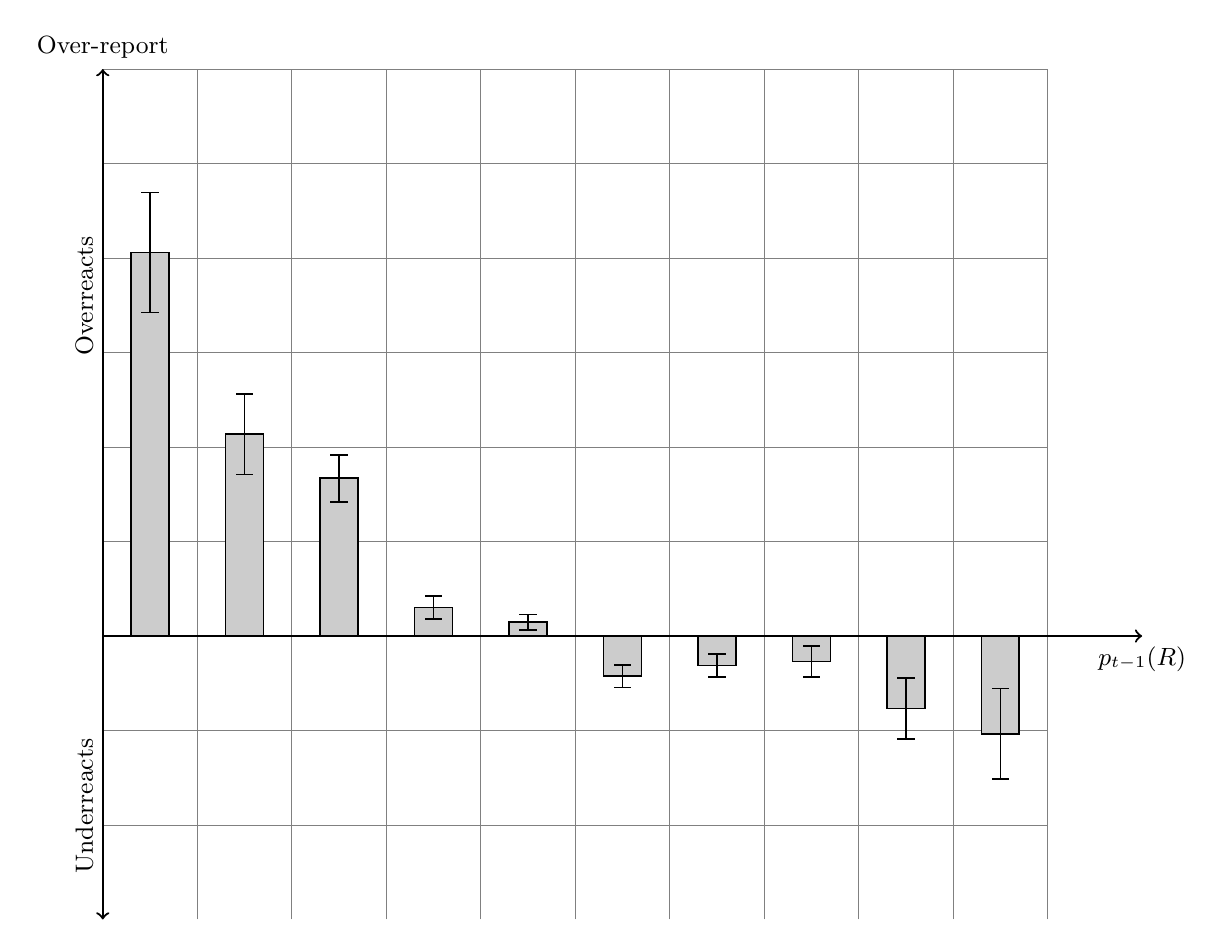
\begin{tikzpicture}[scale=12]
\draw[help lines,step=0.1] (0,-0.3) grid (1,0.6);
\filldraw[opaque,white!80!black] (0.03,0) rectangle (0.07,0.4058);
\draw[line width=0.6] (0.03,0) rectangle (0.07,0.4058);
\draw[line width=0.6,|-|] (0.05,0.3416) -- (0.05,0.4701);
\filldraw[opaque,white!80!black] (0.13,0) rectangle (0.17,0.2135);
\draw[line width=0.6] (0.13,0) rectangle (0.17,0.2135);
\draw[line width=0.6,|-|] (0.15,0.1700) -- (0.15,0.2570);
\filldraw[opaque,white!80!black] (0.23,0) rectangle (0.27,0.1669);
\draw[line width=0.6] (0.23,0) rectangle (0.27,0.1669);
\draw[line width=0.6,|-|] (0.25,0.1412) -- (0.25,0.1926);
\filldraw[opaque,white!80!black] (0.33,0) rectangle (0.37,0.0302);
\draw[line width=0.6] (0.33,0) rectangle (0.37,0.0302);
\draw[line width=0.6,|-|] (0.35,0.0173) -- (0.35,0.0431);
\filldraw[opaque,white!80!black] (0.43,0) rectangle (0.47,0.0147);
\draw[line width=0.6] (0.43,0) rectangle (0.47,0.0147);
\draw[line width=0.6,|-|] (0.45,0.0057) -- (0.45,0.0237);
\filldraw[opaque,white!80!black] (0.53,0) rectangle (0.57,-0.0426);
\draw[line width=0.6] (0.53,0) rectangle (0.57,-0.0426);
\draw[line width=0.6,|-|] (0.55,-0.0553) -- (0.55,-0.0299);
\filldraw[opaque,white!80!black] (0.63,0) rectangle (0.67,-0.0311);
\draw[line width=0.6] (0.63,0) rectangle (0.67,-0.0311);
\draw[line width=0.6,|-|] (0.65,-0.0440) -- (0.65,-0.0182);
\filldraw[opaque,white!80!black] (0.73,0) rectangle (0.77,-0.0269);
\draw[line width=0.6] (0.73,0) rectangle (0.77,-0.0269);
\draw[line width=0.6,|-|] (0.75,-0.0443) -- (0.75,-0.0095);
\filldraw[opaque,white!80!black] (0.83,0) rectangle (0.87,-0.0767);
\draw[line width=0.6] (0.83,0) rectangle (0.87,-0.0767);
\draw[line width=0.6,|-|] (0.85,-0.1102) -- (0.85,-0.0432);
\filldraw[opaque,white!80!black] (0.93,0) rectangle (0.97,-0.1034);
\draw[line width=0.6] (0.93,0) rectangle (0.97,-0.1034);
\draw[line width=0.6,|-|] (0.95,-0.1522) -- (0.95,-0.0547);
\draw[line width=0.8,->]  (0,0) -- (1.1,0) node[below] {\small{$p_{t-1}(R)$}};
\draw[line width=0.8,<->] (0,-0.3) -- (0,0.6) node[above] {\small{Over-report}};
\draw (0,0.36) node[above,rotate=90] {\small{Overreacts}};
\draw (0,-0.18) node[above,rotate=90] {\small{Underreacts}};
% ADD THEORY CURVE BELOW
\end{tikzpicture}
}
\subcaption{$(H_{0,0})$: 0 retractions / 0 confirmations}
\end{subfigure}
\hfill
\begin{subfigure}[t]{0.485\textwidth}
\centering
\resizebox{\linewidth}{!}{
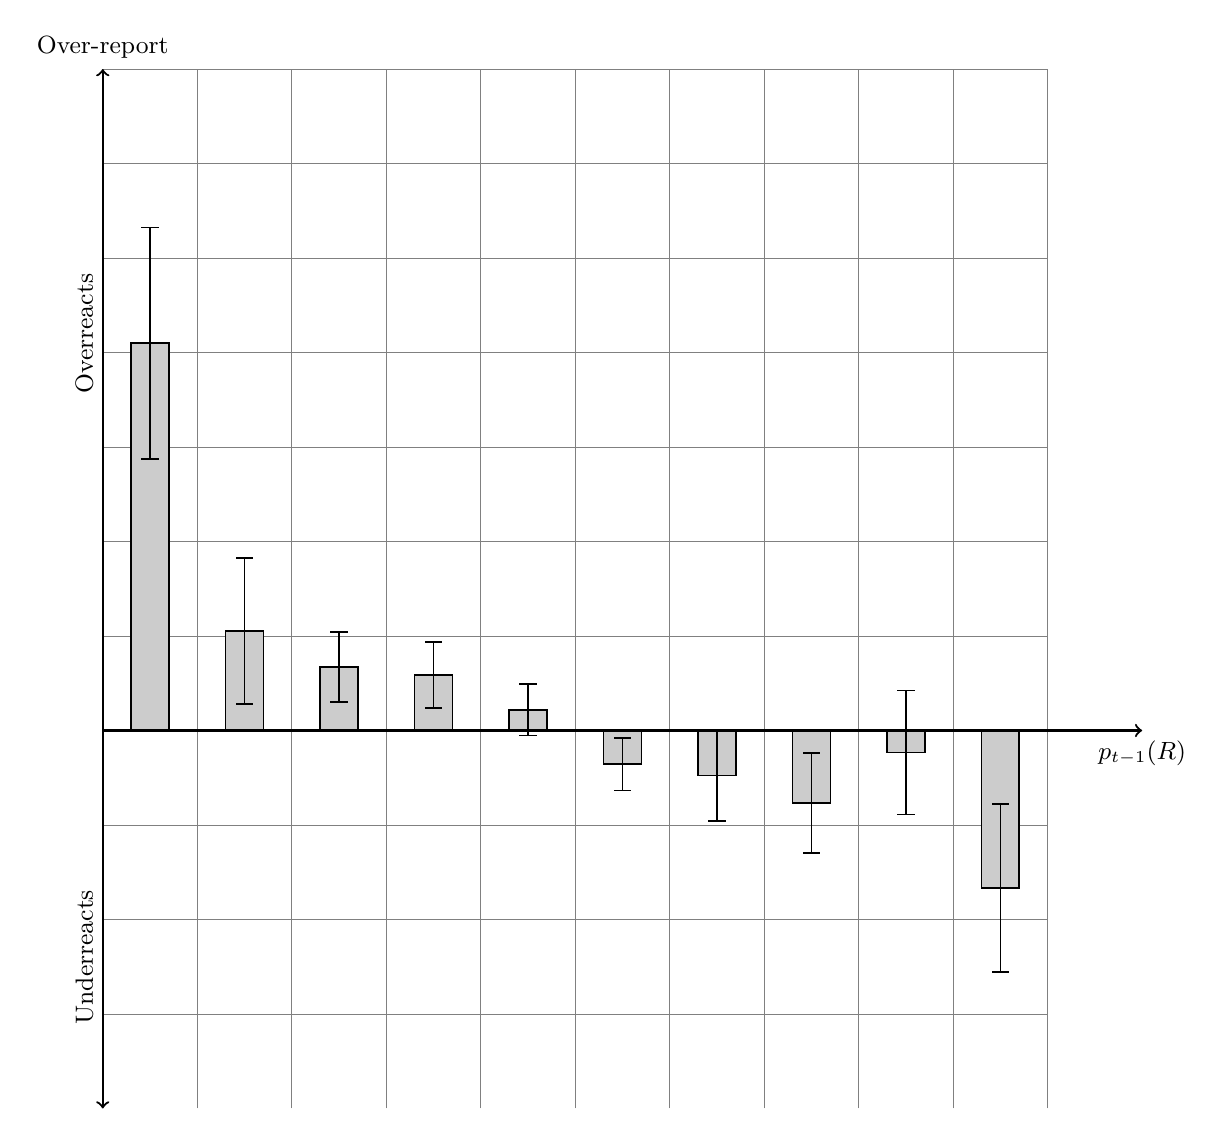
\begin{tikzpicture}[scale=12]
\draw[help lines,step=0.1] (0,-0.4) grid (1,0.7);
\filldraw[opaque,white!80!black] (0.03,0) rectangle (0.07,0.4099);
\draw[line width=0.6] (0.03,0) rectangle (0.07,0.4099);
\draw[line width=0.6,|-|] (0.05,0.2865) -- (0.05,0.5333);
\filldraw[opaque,white!80!black] (0.13,0) rectangle (0.17,0.1053);
\draw[line width=0.6] (0.13,0) rectangle (0.17,0.1053);
\draw[line width=0.6,|-|] (0.15,0.0273) -- (0.15,0.1833);
\filldraw[opaque,white!80!black] (0.23,0) rectangle (0.27,0.0672);
\draw[line width=0.6] (0.23,0) rectangle (0.27,0.0672);
\draw[line width=0.6,|-|] (0.25,0.0293) -- (0.25,0.1051);
\filldraw[opaque,white!80!black] (0.33,0) rectangle (0.37,0.0587);
\draw[line width=0.6] (0.33,0) rectangle (0.37,0.0587);
\draw[line width=0.6,|-|] (0.35,0.0227) -- (0.35,0.0947);
\filldraw[opaque,white!80!black] (0.43,0) rectangle (0.47,0.0220);
\draw[line width=0.6] (0.43,0) rectangle (0.47,0.0220);
\draw[line width=0.6,|-|] (0.45,-0.0061) -- (0.45,0.0502);
\filldraw[opaque,white!80!black] (0.53,0) rectangle (0.57,-0.0358);
\draw[line width=0.6] (0.53,0) rectangle (0.57,-0.0358);
\draw[line width=0.6,|-|] (0.55,-0.0643) -- (0.55,-0.0073);
\filldraw[opaque,white!80!black] (0.63,0) rectangle (0.67,-0.0476);
\draw[line width=0.6] (0.63,0) rectangle (0.67,-0.0476);
\draw[line width=0.6,|-|] (0.65,-0.0969) -- (0.65,0.0017);
\filldraw[opaque,white!80!black] (0.73,0) rectangle (0.77,-0.0767);
\draw[line width=0.6] (0.73,0) rectangle (0.77,-0.0767);
\draw[line width=0.6,|-|] (0.75,-0.1303) -- (0.75,-0.0231);
\filldraw[opaque,white!80!black] (0.83,0) rectangle (0.87,-0.0232);
\draw[line width=0.6] (0.83,0) rectangle (0.87,-0.0232);
\draw[line width=0.6,|-|] (0.85,-0.0899) -- (0.85,0.0434);
\filldraw[opaque,white!80!black] (0.93,0) rectangle (0.97,-0.1666);
\draw[line width=0.6] (0.93,0) rectangle (0.97,-0.1666);
\draw[line width=0.6,|-|] (0.95,-0.2562) -- (0.95,-0.0770);
\draw[line width=0.8,->]  (0,0) -- (1.1,0) node[below] {\small{$p_{t-1}(R)$}};
\draw[line width=0.8,<->] (0,-0.4) -- (0,0.7) node[above] {\small{Over-report}};
\draw (0,0.42) node[above,rotate=90] {\small{Overreacts}};
\draw (0,-0.24) node[above,rotate=90] {\small{Underreacts}};
% ADD THEORY CURVE BELOW
\end{tikzpicture}
}
\subcaption{$(H_{1,0})$: 1 retraction / 0 confirmations}
\end{subfigure}
\\[1.5ex]
\begin{subfigure}[t]{0.485\textwidth}
\centering
\resizebox{\linewidth}{!}{
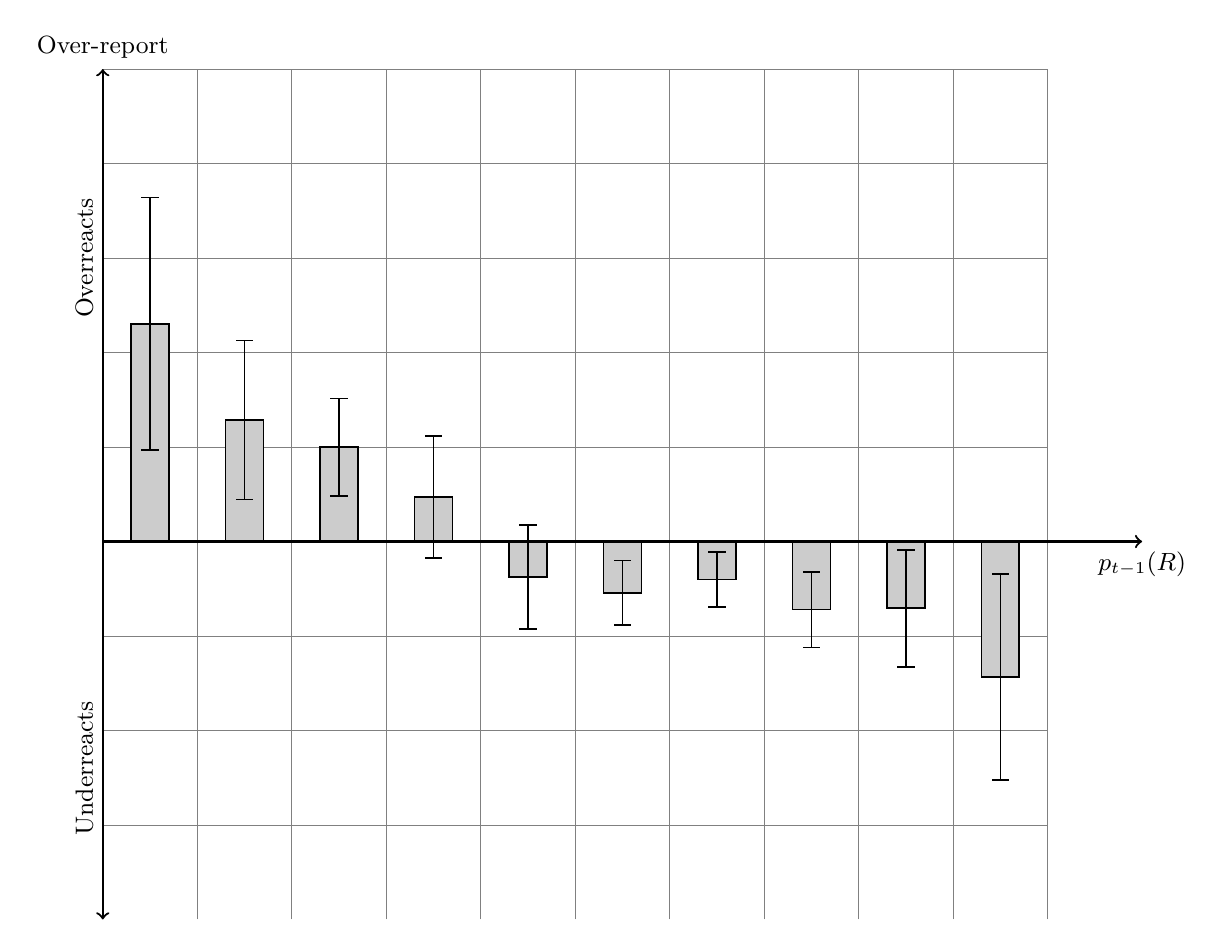
\begin{tikzpicture}[scale=12]
\draw[help lines,step=0.1] (0,-0.4) grid (1,0.5);
\filldraw[opaque,white!80!black] (0.03,0) rectangle (0.07,0.2304);
\draw[line width=0.6] (0.03,0) rectangle (0.07,0.2304);
\draw[line width=0.6,|-|] (0.05,0.0959) -- (0.05,0.3650);
\filldraw[opaque,white!80!black] (0.13,0) rectangle (0.17,0.1286);
\draw[line width=0.6] (0.13,0) rectangle (0.17,0.1286);
\draw[line width=0.6,|-|] (0.15,0.0435) -- (0.15,0.2138);
\filldraw[opaque,white!80!black] (0.23,0) rectangle (0.27,0.0997);
\draw[line width=0.6] (0.23,0) rectangle (0.27,0.0997);
\draw[line width=0.6,|-|] (0.25,0.0472) -- (0.25,0.1522);
\filldraw[opaque,white!80!black] (0.33,0) rectangle (0.37,0.0472);
\draw[line width=0.6] (0.33,0) rectangle (0.37,0.0472);
\draw[line width=0.6,|-|] (0.35,-0.0183) -- (0.35,0.1127);
\filldraw[opaque,white!80!black] (0.43,0) rectangle (0.47,-0.0377);
\draw[line width=0.6] (0.43,0) rectangle (0.47,-0.0377);
\draw[line width=0.6,|-|] (0.45,-0.0936) -- (0.45,0.0182);
\filldraw[opaque,white!80!black] (0.53,0) rectangle (0.57,-0.0543);
\draw[line width=0.6] (0.53,0) rectangle (0.57,-0.0543);
\draw[line width=0.6,|-|] (0.55,-0.0894) -- (0.55,-0.0191);
\filldraw[opaque,white!80!black] (0.63,0) rectangle (0.67,-0.0401);
\draw[line width=0.6] (0.63,0) rectangle (0.67,-0.0401);
\draw[line width=0.6,|-|] (0.65,-0.0703) -- (0.65,-0.0099);
\filldraw[opaque,white!80!black] (0.73,0) rectangle (0.77,-0.0720);
\draw[line width=0.6] (0.73,0) rectangle (0.77,-0.0720);
\draw[line width=0.6,|-|] (0.75,-0.1129) -- (0.75,-0.0312);
\filldraw[opaque,white!80!black] (0.83,0) rectangle (0.87,-0.0707);
\draw[line width=0.6] (0.83,0) rectangle (0.87,-0.0707);
\draw[line width=0.6,|-|] (0.85,-0.1335) -- (0.85,-0.0079);
\filldraw[opaque,white!80!black] (0.93,0) rectangle (0.97,-0.1436);
\draw[line width=0.6] (0.93,0) rectangle (0.97,-0.1436);
\draw[line width=0.6,|-|] (0.95,-0.2534) -- (0.95,-0.0338);
\draw[line width=0.8,->]  (0,0) -- (1.1,0) node[below] {\small{$p_{t-1}(R)$}};
\draw[line width=0.8,<->] (0,-0.4) -- (0,0.5) node[above] {\small{Over-report}};
\draw (0,0.30) node[above,rotate=90] {\small{Overreacts}};
\draw (0,-0.24) node[above,rotate=90] {\small{Underreacts}};
% ADD THEORY CURVE BELOW
\end{tikzpicture}
}
\subcaption{$(H_{0,1})$: 0 retractions / 1 confirmation}
\end{subfigure}
\hfill
\begin{subfigure}[t]{0.485\textwidth}
\centering
\resizebox{\linewidth}{!}{
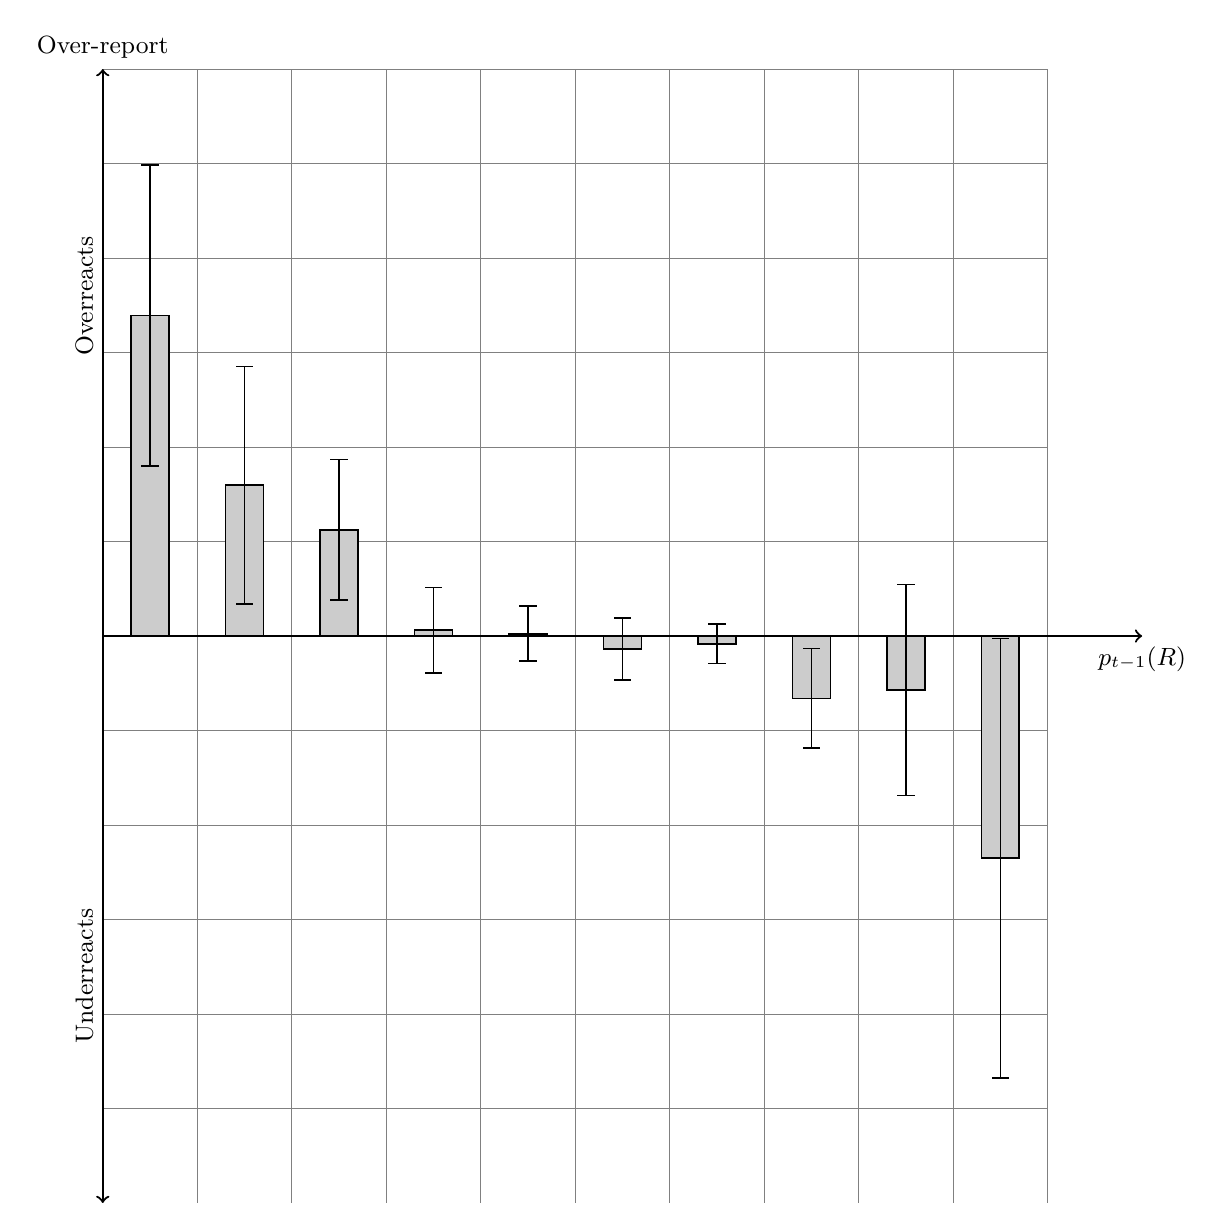
\begin{tikzpicture}[scale=12]
\draw[help lines,step=0.1] (0,-0.6) grid (1,0.6);
\filldraw[opaque,white!80!black] (0.03,0) rectangle (0.07,0.3392);
\draw[line width=0.6] (0.03,0) rectangle (0.07,0.3392);
\draw[line width=0.6,|-|] (0.05,0.1790) -- (0.05,0.4995);
\filldraw[opaque,white!80!black] (0.13,0) rectangle (0.17,0.1596);
\draw[line width=0.6] (0.13,0) rectangle (0.17,0.1596);
\draw[line width=0.6,|-|] (0.15,0.0328) -- (0.15,0.2863);
\filldraw[opaque,white!80!black] (0.23,0) rectangle (0.27,0.1123);
\draw[line width=0.6] (0.23,0) rectangle (0.27,0.1123);
\draw[line width=0.6,|-|] (0.25,0.0370) -- (0.25,0.1876);
\filldraw[opaque,white!80!black] (0.33,0) rectangle (0.37,0.0062);
\draw[line width=0.6] (0.33,0) rectangle (0.37,0.0062);
\draw[line width=0.6,|-|] (0.35,-0.0401) -- (0.35,0.0524);
\filldraw[opaque,white!80!black] (0.43,0) rectangle (0.47,0.0024);
\draw[line width=0.6] (0.43,0) rectangle (0.47,0.0024);
\draw[line width=0.6,|-|] (0.45,-0.0276) -- (0.45,0.0325);
\filldraw[opaque,white!80!black] (0.53,0) rectangle (0.57,-0.0136);
\draw[line width=0.6] (0.53,0) rectangle (0.57,-0.0136);
\draw[line width=0.6,|-|] (0.55,-0.0476) -- (0.55,0.0203);
\filldraw[opaque,white!80!black] (0.63,0) rectangle (0.67,-0.0084);
\draw[line width=0.6] (0.63,0) rectangle (0.67,-0.0084);
\draw[line width=0.6,|-|] (0.65,-0.0301) -- (0.65,0.0134);
\filldraw[opaque,white!80!black] (0.73,0) rectangle (0.77,-0.0660);
\draw[line width=0.6] (0.73,0) rectangle (0.77,-0.0660);
\draw[line width=0.6,|-|] (0.75,-0.1195) -- (0.75,-0.0125);
\filldraw[opaque,white!80!black] (0.83,0) rectangle (0.87,-0.0571);
\draw[line width=0.6] (0.83,0) rectangle (0.87,-0.0571);
\draw[line width=0.6,|-|] (0.85,-0.1696) -- (0.85,0.0554);
\filldraw[opaque,white!80!black] (0.93,0) rectangle (0.97,-0.2351);
\draw[line width=0.6] (0.93,0) rectangle (0.97,-0.2351);
\draw[line width=0.6,|-|] (0.95,-0.4683) -- (0.95,-0.0019);
\draw[line width=0.8,->]  (0,0) -- (1.1,0) node[below] {\small{$p_{t-1}(R)$}};
\draw[line width=0.8,<->] (0,-0.6) -- (0,0.6) node[above] {\small{Over-report}};
\draw (0,0.36) node[above,rotate=90] {\small{Overreacts}};
\draw (0,-0.36) node[above,rotate=90] {\small{Underreacts}};
% ADD THEORY CURVE BELOW
\end{tikzpicture}
}
\subcaption{$(H_{2,0})$: 2 retractions / 0 confirmations}
\end{subfigure}
\\[1.5ex]
\begin{subfigure}[t]{0.485\textwidth}
\centering
\resizebox{\linewidth}{!}{
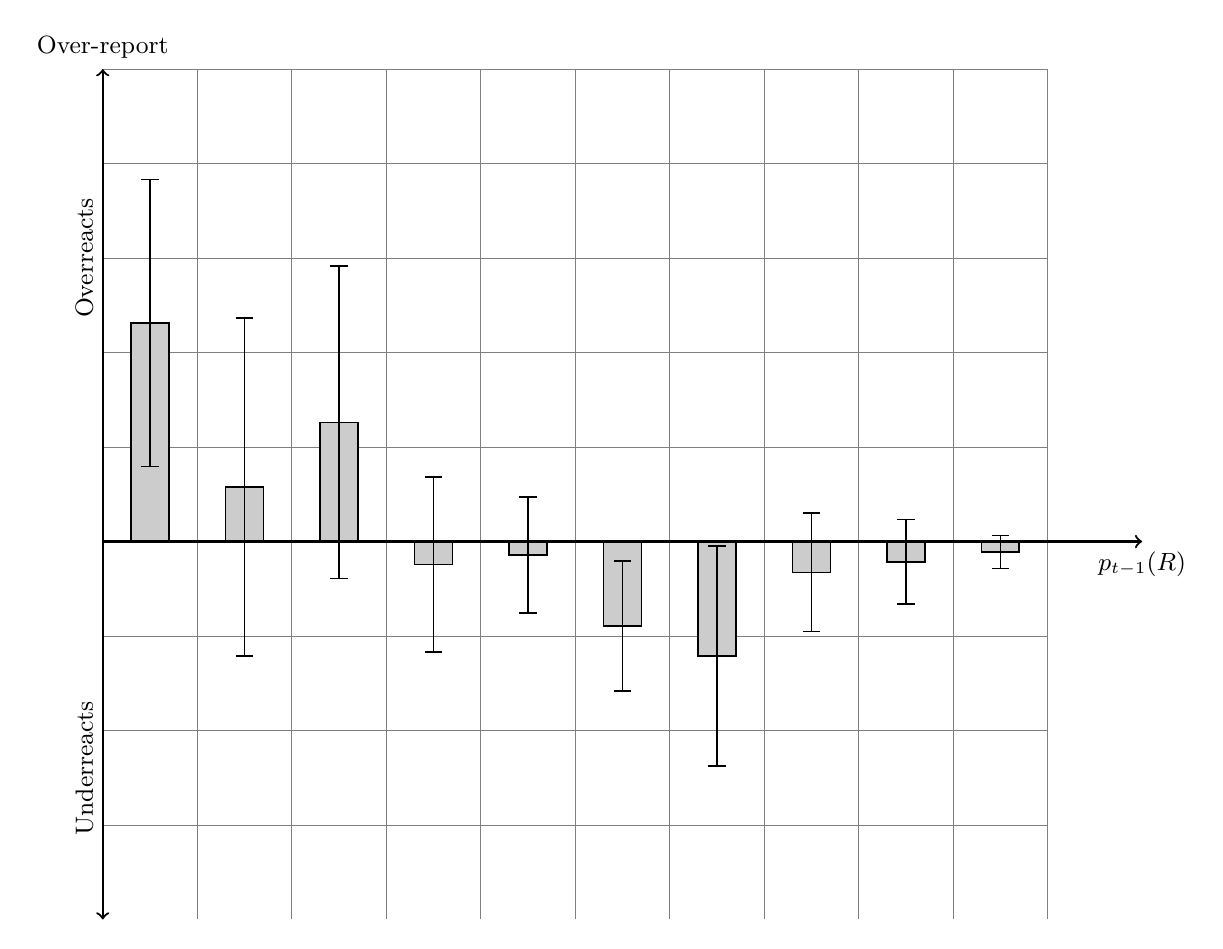
\begin{tikzpicture}[scale=12]
\draw[help lines,step=0.1] (0,-0.4) grid (1,0.5);
\filldraw[opaque,white!80!black] (0.03,0) rectangle (0.07,0.2314);
\draw[line width=0.6] (0.03,0) rectangle (0.07,0.2314);
\draw[line width=0.6,|-|] (0.05,0.0786) -- (0.05,0.3841);
\filldraw[opaque,white!80!black] (0.13,0) rectangle (0.17,0.0575);
\draw[line width=0.6] (0.13,0) rectangle (0.17,0.0575);
\draw[line width=0.6,|-|] (0.15,-0.1222) -- (0.15,0.2373);
\filldraw[opaque,white!80!black] (0.23,0) rectangle (0.27,0.1261);
\draw[line width=0.6] (0.23,0) rectangle (0.27,0.1261);
\draw[line width=0.6,|-|] (0.25,-0.0401) -- (0.25,0.2923);
\filldraw[opaque,white!80!black] (0.33,0) rectangle (0.37,-0.0243);
\draw[line width=0.6] (0.33,0) rectangle (0.37,-0.0243);
\draw[line width=0.6,|-|] (0.35,-0.1176) -- (0.35,0.0689);
\filldraw[opaque,white!80!black] (0.43,0) rectangle (0.47,-0.0143);
\draw[line width=0.6] (0.43,0) rectangle (0.47,-0.0143);
\draw[line width=0.6,|-|] (0.45,-0.0767) -- (0.45,0.0482);
\filldraw[opaque,white!80!black] (0.53,0) rectangle (0.57,-0.0896);
\draw[line width=0.6] (0.53,0) rectangle (0.57,-0.0896);
\draw[line width=0.6,|-|] (0.55,-0.1591) -- (0.55,-0.0200);
\filldraw[opaque,white!80!black] (0.63,0) rectangle (0.67,-0.1210);
\draw[line width=0.6] (0.63,0) rectangle (0.67,-0.1210);
\draw[line width=0.6,|-|] (0.65,-0.2382) -- (0.65,-0.0039);
\filldraw[opaque,white!80!black] (0.73,0) rectangle (0.77,-0.0327);
\draw[line width=0.6] (0.73,0) rectangle (0.77,-0.0327);
\draw[line width=0.6,|-|] (0.75,-0.0962) -- (0.75,0.0308);
\filldraw[opaque,white!80!black] (0.83,0) rectangle (0.87,-0.0215);
\draw[line width=0.6] (0.83,0) rectangle (0.87,-0.0215);
\draw[line width=0.6,|-|] (0.85,-0.0672) -- (0.85,0.0241);
\filldraw[opaque,white!80!black] (0.93,0) rectangle (0.97,-0.0112);
\draw[line width=0.6] (0.93,0) rectangle (0.97,-0.0112);
\draw[line width=0.6,|-|] (0.95,-0.0295) -- (0.95,0.0071);
\draw[line width=0.8,->]  (0,0) -- (1.1,0) node[below] {\small{$p_{t-1}(R)$}};
\draw[line width=0.8,<->] (0,-0.4) -- (0,0.5) node[above] {\small{Over-report}};
\draw (0,0.30) node[above,rotate=90] {\small{Overreacts}};
\draw (0,-0.24) node[above,rotate=90] {\small{Underreacts}};
% ADD THEORY CURVE BELOW
\end{tikzpicture}
}
\subcaption{$(H_{0,2})$: 0 retractions / 2 confirmations}
\end{subfigure}
\hfill
\begin{subfigure}[t]{0.485\textwidth}
\centering
\resizebox{\linewidth}{!}{
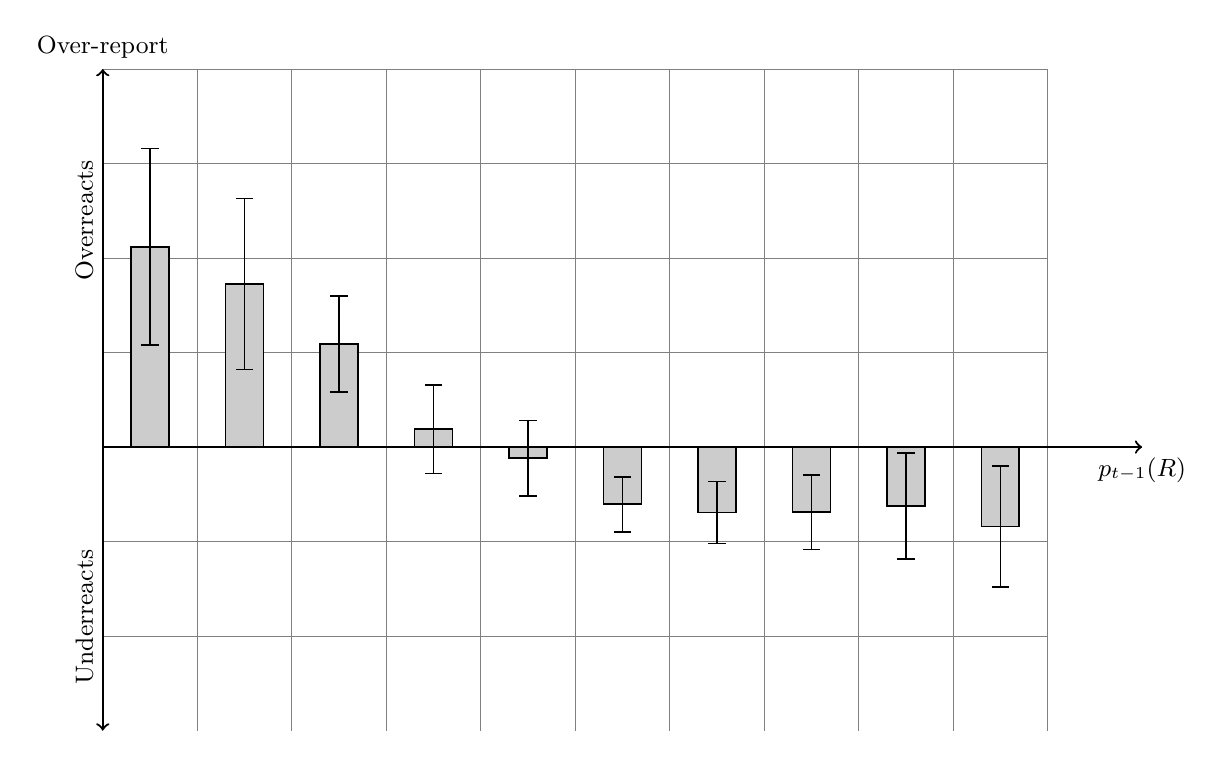
\begin{tikzpicture}[scale=12]
\draw[help lines,step=0.1] (0,-0.3) grid (1,0.4);
\filldraw[opaque,white!80!black] (0.03,0) rectangle (0.07,0.2119);
\draw[line width=0.6] (0.03,0) rectangle (0.07,0.2119);
\draw[line width=0.6,|-|] (0.05,0.1071) -- (0.05,0.3168);
\filldraw[opaque,white!80!black] (0.13,0) rectangle (0.17,0.1726);
\draw[line width=0.6] (0.13,0) rectangle (0.17,0.1726);
\draw[line width=0.6,|-|] (0.15,0.0811) -- (0.15,0.2640);
\filldraw[opaque,white!80!black] (0.23,0) rectangle (0.27,0.1089);
\draw[line width=0.6] (0.23,0) rectangle (0.27,0.1089);
\draw[line width=0.6,|-|] (0.25,0.0573) -- (0.25,0.1605);
\filldraw[opaque,white!80!black] (0.33,0) rectangle (0.37,0.0189);
\draw[line width=0.6] (0.33,0) rectangle (0.37,0.0189);
\draw[line width=0.6,|-|] (0.35,-0.0289) -- (0.35,0.0668);
\filldraw[opaque,white!80!black] (0.43,0) rectangle (0.47,-0.0117);
\draw[line width=0.6] (0.43,0) rectangle (0.47,-0.0117);
\draw[line width=0.6,|-|] (0.45,-0.0525) -- (0.45,0.0291);
\filldraw[opaque,white!80!black] (0.53,0) rectangle (0.57,-0.0606);
\draw[line width=0.6] (0.53,0) rectangle (0.57,-0.0606);
\draw[line width=0.6,|-|] (0.55,-0.0906) -- (0.55,-0.0306);
\filldraw[opaque,white!80!black] (0.63,0) rectangle (0.67,-0.0693);
\draw[line width=0.6] (0.63,0) rectangle (0.67,-0.0693);
\draw[line width=0.6,|-|] (0.65,-0.1030) -- (0.65,-0.0355);
\filldraw[opaque,white!80!black] (0.73,0) rectangle (0.77,-0.0690);
\draw[line width=0.6] (0.73,0) rectangle (0.77,-0.0690);
\draw[line width=0.6,|-|] (0.75,-0.1093) -- (0.75,-0.0287);
\filldraw[opaque,white!80!black] (0.83,0) rectangle (0.87,-0.0625);
\draw[line width=0.6] (0.83,0) rectangle (0.87,-0.0625);
\draw[line width=0.6,|-|] (0.85,-0.1197) -- (0.85,-0.0053);
\filldraw[opaque,white!80!black] (0.93,0) rectangle (0.97,-0.0840);
\draw[line width=0.6] (0.93,0) rectangle (0.97,-0.0840);
\draw[line width=0.6,|-|] (0.95,-0.1491) -- (0.95,-0.0189);
\draw[line width=0.8,->]  (0,0) -- (1.1,0) node[below] {\small{$p_{t-1}(R)$}};
\draw[line width=0.8,<->] (0,-0.3) -- (0,0.4) node[above] {\small{Over-report}};
\draw (0,0.24) node[above,rotate=90] {\small{Overreacts}};
\draw (0,-0.18) node[above,rotate=90] {\small{Underreacts}};
% ADD THEORY CURVE BELOW
\end{tikzpicture}
}
\subcaption{$(H_{1,1})$: 1 retraction / 1 confirmation}
\end{subfigure}
